% Preamble
\documentclass[11pt]{article}
\usepackage{braket}
\usepackage{graphicx}
\usepackage[margin=1in]{geometry}

\usepackage{makeidx}  % allows for indexgeneration
\usepackage{ifpdf}
\usepackage{url}


\title{Elementary Cellular Automata as Non-Cryptographic Hash Functions}
\date{May 2025}
\author{Daniel McKinley}

% Document
\begin{document}

\maketitle

\section{Introduction}

Elementary cellular automata (ECA) are 8 bit truth tables (Wolfram codes) done linearly in parallel. \cite{Wolfram}
Here a subset of 8 of the 256 ECA rules are explored as a non-cryptographic hash function using a lossy compression error-minimization function. The hash's key properties are that the codewords are unique and evenly distributed, has an inverse, and that hashed data can be operated on without inversion and without the original data.  The loops parallel the nested $2^n$ structure of the Fast Fourier Transform (FFT) and Fast Walsh-Hadamard Transform and the Hadamard parity of a codeword can be substituted in the inversion process. General algorithm outline, specific ECA rules, and aggregate properties are discussed. It is implemented in Java at \cite{mygit} and applied to bitmap images along with more images and gifs at the website.\\

\section{Main Algorithm}
\begin{center}

There are $2^{16}=65536$ binary 4x4 arrays\\
 Where there are $2^4$ possible $row_0$ neighborhoods for a given ECA rule\\
 Each of these 16 input-ECAoutput arrays are scored for errors by\\
\[  \sum_{r=0}^{3} \sum_{c=0}^{3} 2^r ( compressionAttempt_{r c} \oplus original_{r c}) \]\\
 The minimizing and maximizing values of all possible inputs\\
 are noted as the codeword pair of the original binary matrix\\
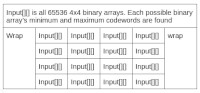
\includegraphics{inputGrid}\\
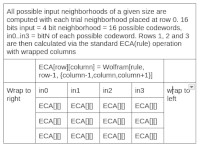
\includegraphics{ecaGrid}\\
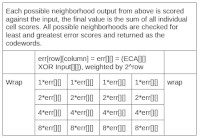
\includegraphics{errorGrid}\\
\end{center}
The hash algorithm is a kind of lossy compression that operates on 4x4 wrapped cells of binary input data. Within each cell, row 0 is the input neighborhood and the ECA rule's output is calculated for rows 1,2 and 3. All 16 possible row 0 inputs are calculated and then scored where each bitwise discrepancy between the codeword's output and the input is summed with a weight of $2^row$. The input neighborhoods that minimize and maximize the error score are noted as the codeword pair for that 4x4 input and each codeword is 4 bits. Doing this procedure for all  $2^{16}=65536$ possible 4x4 input neighborhoods produces a truth table for a particular ECA rule.\\

Having produced a truth table as above for a given ECA rule, it is applied to a bitmap image as follows. For every (wrapped) (row,column) location in the input, the 4x4 local cell is the hexadecimal of that location and its right, down, and diagonal right-down neighbors $2^d$ away, $(row,column)..((row+2^d),(column+2^d))$  where d is depth of iteration. The value is replace with the respective minimizing or maximizing codewords. This comparing of neighbors of powers of 2 distance away is the same flow chart as the FFT and Fast Walsh Transform with reminimizations instead of sums and/or products at every level of recursion. These exponential neighborhood expansions guarantee the avalanche property in $log_2(size)$ time. Using the subset of ECA rules described below, there is only one set of codewords that describe it.\\
\begin{center}
Below is a Fast Walsh-AlgorithmCode.Hadamard Example \cite{enwiki:1261916659}\\
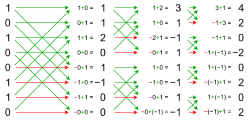
\includegraphics{FastWalshHadamard}\\
If you did the above with the powers of 2 in reverse order you would get this. \\
This the 1 dim version, and instead of a sum term it's a rehash.\\ 
Find the codewords of the codewords, twice as far apart each time.\\
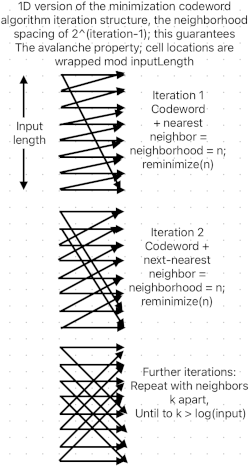
\includegraphics{AlgoStruct}\\
\end{center}

This transformation is perfectly invertible when using a complete minMax codeword rule set of 16. A single rule of the positive 8-tuple of the below is lossy, with an error rate of 3/8, however if the input is hashed as a set with every rule in the tuple, a voting process produces the inverse and the loss rate becomes 0. With a rectangular bitmap inverse, the voting process is the overlapping codewords for all 8 of the rules in the subset as well as the 8 max codewords together make a weighted vote on the inverse of the algorithm. Each codeword is that location's best guess on its neighborhood and each location is part of at least 4 neighborhoods at each iteration, twice as far apart each time. The cell's best-gues output is weighted by its relative row or column and added to its location's tally of votes. At the end if the sum of the weighted votes is positive then it becomes 0, if it is negative it becomes 1. \\

This algorithm both minimizes the errorScore in a lossy compression, and maximize the errorScore. There are dual min-max versions of most variables in the implementation. \\

\section{A subset of the 0-255 ECA}

Within the 256 ECA rules, there are 8 [0,15,51,85,170,204,240,255] that have the properties of unique codewords for any given input as well as a perfectly even distribution of codewords across the 65536 neighborhoods in the truth table. 0 and 255 are included because in the 4 rows of the output matrix, 1 is neighborhood input and 3 are output, and so still produce an errorScore and therefore a unique solution. These properties apply to these rules with both errorScore minimization and errorScore maximization. \\

There is another overlapping subset of 8, [0,15,85,90,165,170,240,255] that when the errorScore weight is $2^{row}$ rather than $2^{column}$ like the above, the same properties apply. The codewords are distributed perfectly evenly, there are unique solutions for every input, and has a minimizing and a maximizing codeword set. These lists share a few members with the XOR-additive list. \cite{xorAdditive}. Most properties apply equally to both with a few exceptions.\\

\section{Hash properties}

This algorithm is at least collision resistant with an extra loop and array space in memory guaranteeing no collisions. On their own codeword tuples are not distinct for a given bitmap even if an individual codeword is; however wrapping the codewords over themselves the tuple becomes unique; the rare artificially produced small neighborhood collisions disappeared when the same sample was wrapped, eliminating the possibility of any collision. An extra wrap loop on each cell adds factor of 16 in both time and memory for an absolute no-collision set. Without that loop, random testing of collisions produced an one in a hundred trillion on a 5x5 matrix that disappeared when the neighborhood was wrapped. Small scale local collisions are a possibility, large scale collisions are unlikely, and optionally no collisions.\\

All 32 Wolfram codes in the 4 minMax row-column sets of 8 have an even distribution of codewords. Each 0..15 codeword is used 4096 times, distributed relatively evenly across the 65536 possible binary 4x4 cells.\\

Hashed input can be operated on without the original input and without inverting it. Because the ECA rules in the 8-subset are linear, if you take any 2 of 16 codeword-generated 4x4 cells and OR them together and reminimize, the result is the same as the original two codewords ANDed together.  This shift of logic operations within a hash is uniform within an ECA rule hash and extends to any depth of iteration the hash algorithm transforms not only the input data but also the relative logic gate. For example if I want to retroactively apply a bitmask to a hashed image or IP address without the original image and without inversion, hash the bitmask and lookup the appropriate logic gate tranformation between the hashed image and the hashed bitmask.\\

Internalized hash logic operation transformations operate somewhat differently for the row and error scored subsets. The truth tables are generated by brute force taking all codeword pairs generating 4x4 cells that are taken against all logic operations across all 32 minMax 8 subsets and eliminating all logic gates that do not reproduce the same operation on the codewords leaving the working logic gate. The row weighted errorScore truth tables are more straightforward to generate, requiring only a single operation per truth table, while the column weighted errorScore truth tables are granular and require an individual gate per cell per truth table and thus an extra array and loop per truth table.\\

This algorithm displays some avalanche properties. The threshold for testing is when every pixel hexadecimal set has had an opportunity to influence every other pixel, or $log_2(imageWidth)$ or $log_2(imageHeight)$, whichever is greater. Experimentally changing small numbers of pixels and running the required number of iterations produce the possible property. What happens at that point is that triplets within a rule subset display a substantial number of changes on alternating iterations. On even iterations within the min codeword set, 15, 51, and 85 have many changes while 170, 204, and 240 don't, and the opposite on odd iterations. The same alternating happens with the column weighted errorScore set triplets to a lesser extent.\\

This algorithm can be used to make any sized hash. This hash is implemented to either hash-in-place so that the data stays the same size or as compression with the data size quartering each iteration. To implement any size output, first hash to the avalanche point as the fixed data size version, then as compression to the size desired and/or pad with zeroes. Rather than padding with zeroes one can use an inversion to expand the hash to a larger size, however inversion is more computationally expensive than compression.\\

\section{Implementation, Testing, and Performance}

The algorithm is prototyped on 4-byte, 3-byte, and 2-byte RGB *.bmp bitmap files, including the first several images which come from a Linux screenshot then into *.bmp by GIMP. The program converts the image's raster in a rectangular hexadecimal array. Animated *.gif files are available at my website. You can see the areas of the image cloning itself 2 by 2 and slowly dissolving into avalanche territory that eventually just looks like noise everywhere. The current image was chosen because you can clearly see parts of the image doubling itself as the avalanche property slowly takes over. The code works with any size bitmap. Future work on the project would include other image formats as it is a color code hexadecimal conversion. \\

Testing\\


\begin{center}
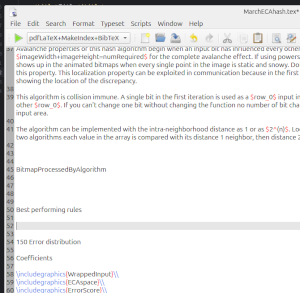
\includegraphics{testScreenshot}\\
Original Image\\
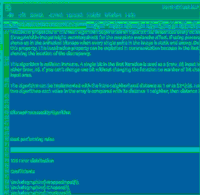
\includegraphics{processedDepth3}\\
Frame 3\\

\includegraphics{processedDepth6}\\
Frame 6\\
\end{center}

\section{Other rules, shapes, and sizes}

The weight in the errorScore sum can be $2^{row}$ or $2^{column}$, both produce the same set of 8 tuples with the unique solution and even distribution properties, though other ECA rules' properties don't necessarily carry over. This transposition and reflections across an axis may be enough to produce unique tuples without the loop, however checking this is ongoing.\\

The size of the input array can be easily be any power of 2 squared. Within this prototype project, calculation of Wolfram code lengths of $2^{16}$ using all 4x4 binary grids are acceptable, lengths of $2^{64}$ using 8x8 grids would be challenging at this point. At size 8 there are $2^8=256$ possible codewords, which means that while you can't calculate the whole truth table at once you can calculate the codewords individually on the spot. The 8 tuple's uniqueness and distribution properties probably apply at larger sizes, it may not; it is only exhaustively tested for size 4 and size 8 is only randomly spot-checked. The internal hash logic transforms can still be easily calculated for size 8 because you only have to work with codewords rather than the entire set of inputs. Sizes other than 4 and 8 are not considered here.\\

Out of the other 0-255 ECA rules, some do better than these particular 8 at lossy compression, losing only 3/16 bits instead of 6/16 bits with these 8. In particular the Pascal rules 90, 165, 102, 153, 105, 150 rank near the top, connected to several these 8 via the property of XOR-additiveness (cite wolfram atlas). However none outside of these 8 have unique solutions or even distributions in either row or column weighted, maxxed or minned.\\

\section{Rule 150}

If while running this algorithm for rule 150 you produce a heat map of the errors in reconstructing the lossy compression, you get this. To seven binary digits, five past the decimal place, Phi and Pi show up in these ratios. Seven binary digits is a 2\% error rate. Seven digits is enough for an ASCII operation. Precision to seven decimal places shows up here and in reconstructing the 8-tuples above. If you label a five point star and proceed backwards starting at 0, you get \{3,1,4,2,0\} which is roughly the same seven digit precision. Some of those mentioned here are seven binary digits some are accurate to nine. While seven digits by itself is not impressive, 7 digits across three constants is notable.\\

\noindent rule 150\\

\noindent minErrorMap\\
29482 29482 29476 29464 \\
30940 30904 30958 30958 \\
17486 17486 17516 17576 \\
5532 5592 5502 5502 \\

\noindent minProportions[][]\\
1.0000 0.9527 1.6828 5.3283 \\
1.0497 1.0000 1.7664 5.5929 \\
0.5942 0.5661 1.0000 3.1663 \\
0.1877 0.1788 0.3158 1.0000 \\
2.621312044429018\\

\noindent a = row2 / row 3 = 3.166305133767173\\
a = (row2 / row 3) - PI = 0.024712480177379703\\
accurate to the binary -5 place\\

\noindent b = row1 / row 0 = 1.0496675261229476\\
b = (row1 / row 1) - (PI/3) = 0.002469974926349927\\
accurate to the binary -9 place\\

\noindent c = (row0+row1)/(row2+row3) = 2.621312044429018\\
c = (row0+row1)/(row2+row3) - PhiSquared = 0.003278055679122982\\
accurate to the binary -8 place\\

\noindent Throw in the 1's and 2's place makes for 7, 11, and 10 accurate digits\\
If you compare that accuracy to the method of computing pi by the edges of increasing numbers of triangles\\
it takes dividing 2Pi into 32 triangles to get 7 digits. If takes 32 iterations of the Wallis product\\

\bibliographystyle{plain}
\bibliography{HashBib.bib}

\end{document}